\documentclass[a4paper]{article}
\usepackage{vntex}
\usepackage{amsmath}
\usepackage{blindtext}
\usepackage[english]{babel}
\usepackage{minted}
\usepackage{a4wide,amssymb,epsfig,latexsym,multicol,array,hhline,fancyhdr}
\usepackage{booktabs}
\usepackage{lastpage}
\usepackage[lined,boxed,commentsnumbered]{algorithm2e}
\usepackage{enumerate}
\usepackage{makecell}
\usepackage{color}
\usepackage{svg}
\usepackage{graphicx}   % Standard graphics package
\usepackage{enumitem}
\usepackage{tabularx, caption}
\usepackage{multirow}
\usepackage[framemethod=tikz]{mdframed}  % For highlighting paragraph backgrounds
\usepackage{multicol}
\usepackage{rotating}
\usepackage{geometry}
\usepackage{setspace}
\usepackage{tikz}
\usepackage{listings}
\usetikzlibrary{arrows,snakes,backgrounds}
\usepackage{hyperref}
\hypersetup{urlcolor=blue,linkcolor=black,citecolor=black,colorlinks=true}\usepackage{xurl}  % Load the xurl package, which allows line breaks at any character in URLs
\usepackage{hyperref}  % Ensure hyperref is loaded for clickable links
\hypersetup{
    colorlinks=true,
    linkcolor=black,
    filecolor=magenta,      
    urlcolor=blue,
    citecolor=black
}



\everymath{\color{blue}}
\setlength{\headheight}{40pt}
\pagestyle{fancy}
\fancyhead{} % clear all header fields
\fancyhead[L]{
 \begin{tabular}{rl}
    \begin{picture}(25,15)(0,0)
    \put(0,-8){
\includegraphics[width=8mm, height=8mm]{hcmut.png}}
   \end{picture}&
    \begin{tabular}{l}
        \textbf{\bf \ttfamily University of Technology}\\
        \textbf{\bf \ttfamily Faculty of Computer Science and Engineering}
    \end{tabular}     
 \end{tabular}
}
\fancyhead[R]{
    \begin{tabular}{l}
        \tiny \bf \\
        \tiny \bf 
    \end{tabular}  
}
\fancyfoot{} % clear all footer fields
\fancyfoot[L]{\scriptsize \ttfamily \textcolor{blue}{Discrete structure (CO1007) Assignment, Semester 2, Academic year}}
\fancyfoot[R]{\scriptsize \ttfamily Page {\thepage}/\pageref{LastPage}}
\renewcommand{\headrulewidth}{0.3pt}
\renewcommand{\footrulewidth}{0.3pt}

\setcounter{secnumdepth}{4}
\setcounter{tocdepth}{3}
\makeatletter
\newcounter{subsubsubsection}[subsubsection]
\renewcommand\thesubsubsubsection{\thesubsubsection .\@alph\c@subsubsubsection}
\newcommand\subsubsubsection{\@startsection{subsubsubsection}{4}{\z@}%
                                     {-3.25ex\@plus -1ex \@minus -.2ex}%
                                     {1.5ex \@plus .2ex}%
                                     {\normalfont\normalsize\bfseries}}
\newcommand*\l@subsubsubsection{\@dottedtocline{3}{10.0em}{4.1em}}
\newcommand*{\subsubsubsectionmark}[1]{}
\makeatother

\begin{document}

\begin{titlepage}
\begin{center}
\Large Vietnam National University, Ho Chi Minh City \\
\Large University of Technology \\
\Large Faculty of Computer Science and Engineering 
\end{center}

\vspace{1cm}

\begin{figure}[h!]
\begin{center}

\includegraphics[width=4cm]{hcmut.png}
\end{center}
\end{figure}

\vspace{1cm}

\begin{center}
\begin{tabular}{c}
    \multicolumn{1}{l}{\textbf{{\Large DISCRETE STRUCTURE
(CO1007)}}}\\
    ~~\\
    \hline
    \\
    \multicolumn{1}{l}{\textbf{{\Large Assignment }}}\\
    \\
        \textbf{{\LARGE “Traveling Saleman Problem”}}\\
    \\
    \hline
\end{tabular}
\end{center}
\vspace{2cm}

\begin{table}[h]
\begin{tabular}{rrl}
\hspace{3 cm} 
& Instructor(s): & Nguyễn Văn Minh Mẫn, Mahidol University \\
& &  Nguyễn An Khương, CSE-HCMUT \\
& &  Trần Tuấn Anh,CSE-HCMUT \\
& &  Nguyễn Tiến Thịnh, CSE-HCMUT \\
& &  Trần Hồng Tài, CSE-HCMUT \\
& &  Mai Xuân Toàn, CSE-HCMUT \\
& Class: &L05\\
& Student: & Nguyễn Việt Anh - 2210116\\
\end{tabular}
\end{table}
\vspace{1cm}
\begin{center}
\date{\footnotesize\today}
\end{center}
\end{titlepage}

\thispagestyle{empty}

\newpage
\renewcommand{\contentsname}{Table of Contents}
\tableofcontents
\newpage

%%%%%%%%%%%%%%%%%%%%%%%%%%%%%%%%%
\section{Introduction to the Travelling Salesman Problem}
The Travelling Salesman Problem (TSP) is one of the most extensively studied problems in the field of combinatorial optimization. It is defined as follows: given a list of cities and the distances between each pair of cities, what is the shortest possible route that visits each city exactly once and returns to the origin city?

TSP is significant both theoretically and practically. It is an NP-hard problem in computational complexity theory, meaning that there is no known polynomial-time solution for it. Despite this, TSP has numerous practical applications, including logistics, planning, and the manufacturing of microchips.

\subsection{History and Importance}
The Travelling Salesman Problem was first formulated in the 19th century by the Irish mathematician William Rowan Hamilton and the British mathematician Thomas Penyngton Kirkman. Its importance has grown over time due to its applicability in various fields and its role in the development of optimization algorithms and computational complexity theory.

\subsection{Formal Definition}
Formally, the TSP can be described as follows: let \( G = (V, E) \) be a complete graph where \( V \) represents the set of vertices (cities) and \( E \) represents the set of edges (paths between the cities). Each edge \( (i, j) \in E \) has an associated weight \( d(i, j) \), which represents the distance between cities \( i \) and \( j \). The goal is to find a Hamiltonian cycle (a cycle that visits each vertex exactly once and returns to the starting vertex) with the minimum possible total weight.

\subsection{Applications}
The TSP has a wide range of applications:
\begin{itemize}
    \item \textbf{Logistics and Transportation:} Optimizing routes for delivery trucks, mail carriers, and sales representatives.
    \item \textbf{Manufacturing:} Planning the movement of robotic arms in automated assembly lines.
    \item \textbf{Genomics:} Sequencing DNA to minimize errors.
    \item \textbf{Telecommunications:} Optimizing the layout of circuits on a microchip.
\end{itemize}

\subsection{Challenges and Complexity}
The primary challenge of the TSP lies in its computational complexity. As the number of cities increases, possible routes grow factorially, making brute-force solutions impractical for large instances. This has led to the development of various heuristic and approximation algorithms, such as the nearest neighbor algorithm, genetic algorithms, and simulated annealing.

\subsection{Conclusion}
The Travelling Salesman Problem continues to be a central problem in operations research and computer science due to its theoretical significance and practical relevance. Advances in solving TSP have broad implications for optimization and computational theory, making it a fascinating and crucial area of study.

\section{Methods for Solving the Travelling Salesman Problem}
The Travelling Salesman Problem (TSP) is a classic optimization problem that has been approached using various methods. These methods can be broadly classified into exact algorithms, approximation algorithms, and heuristics. Each method has its own advantages and limitations depending on the problem size and specific requirements.

\subsection{Exact Algorithms}
Exact algorithms guarantee to find the optimal solution to the TSP but are generally computationally expensive for large instances. Some of the common exact algorithms include:
\begin{itemize}
    \item \textbf{Dynamic Programming:} The Held-Karp algorithm uses dynamic programming to solve TSP with a time complexity of \(O(n^2 \cdot 2^n)\), where \(n\) is the number of cities.
    \item \textbf{Integer Linear Programming (ILP):} Formulates TSP as a linear program with integer constraints. Solvers like CPLEX or Gurobi can be used to find the optimal solution.
    \item \textbf{Branch and Bound:} A systematic method of solving TSP by exploring all possible routes while pruning suboptimal routes to reduce computation.
\end{itemize}

\subsection{Approximation Algorithms}
Approximation algorithms provide solutions close to the optimal solution with a guarantee of the solution quality. These include:
\begin{itemize}
    \item \textbf{Christofides' Algorithm:} Guarantees a solution within 1.5 times the optimal solution for metric TSP.
    \item \textbf{Nearest Neighbor Algorithm:} Builds a route by repeatedly visiting the nearest unvisited city, though it does not guarantee optimality.
\end{itemize}

\subsection{Heuristics and Metaheuristics}
Heuristics and metaheuristics provide good solutions within a reasonable time frame, often without guarantees of optimality. Common approaches include:
\begin{itemize}
    \item \textbf{Genetic Algorithms:} Uses principles of natural selection to iteratively improve the solution.
    \item \textbf{Simulated Annealing:} Mimics the cooling process of metals to escape local minima and find a good approximation of the global minimum.
    \item \textbf{Ant Colony Optimization:} Simulates the behavior of ants to find optimal paths based on pheromone trails.
\end{itemize}

\subsection{Why Use Branch and Bound?}
The Branch and Bound method is a popular exact algorithm for solving the TSP due to several reasons:
\begin{itemize}
    \item \textbf{Optimality:} It guarantees finding the optimal solution by systematically exploring and evaluating all possible routes.
    \item \textbf{Pruning:} By effectively pruning suboptimal routes early in the search process, it reduces the computational burden compared to brute-force methods.
    \item \textbf{Flexibility:} Branch and Bound can be combined with other techniques, such as heuristics, to improve its efficiency for large instances.
    \item \textbf{General Applicability:} It is not limited to TSP and can be applied to various other combinatorial optimization problems.
\end{itemize}

The Branch and Bound method involves dividing the problem into smaller subproblems (branching) and calculating a bound on the minimum possible cost of any solution within each subproblem. If the bound for a subproblem exceeds the current best-known solution, the subproblem is discarded (pruned). This process continues until the optimal solution is found.\\

In conclusion, while many methods exist for solving the TSP, the choice of method depends on the specific requirements and constraints of the problem. Branch and Bound stand out as a powerful method due to its balance between guaranteeing optimal solutions and reducing computational complexity through effective pruning.


\section{Code and Explaination}
\subsection{Header File - tsm.h}
\begin{minted}[frame=lines,framesep=2mm,baselinestretch=1.2,fontsize=\footnotesize,linenos]{cpp}
#include <iostream>
#include <vector>
#include <algorithm>
#include <climits>
#include <cstring>
#include <string>
#include <fstream>
#ifndef TSM_H
#define TSM_H

using namespace std;
const int MAXN = 20; // Maximum number of cities/nodes
const int MAXINT = -1;
extern int DEM;  // External declaration for the count of recursive calls
extern int COUNT;  // External declaration for the count of better solutions found

// Declarations for the Branch and Bound algorithm functions
void branchBoundHelp(int G[MAXN][MAXN], int n, int startCity, int i, int minCost, int& tmpRes, int& result, 
int tempPath[], int path[], int visited[]);
std::string branchBound(int G[MAXN][MAXN], int n, char start);
std::string Traveling(int G[MAXN][MAXN], int n, char start);

#endif
\end{minted}

\subsection{Implementation File - tsm.cpp}
\begin{minted}[frame=lines,framesep=2mm,baselinestretch=1.2,fontsize=\footnotesize,linenos]{cpp}
#include "tsm.h"

// Global variables
int DEM = 0;  // Counter for the number of recursive calls
int COUNT = 0;  // Counter for the number of times a better solution is found

// Helper function for the Branch and Bound algorithm
// G: adjacency matrix, n: number of cities, startCity: starting city index
// i: current depth in the search tree, minCost: minimum edge cost
// tmpRes: current path cost, result: best path cost so far
// tempPath: current path being explored, path: best path found so far
// visited: array to keep track of visited cities
void branchBoundHelp(int G[MAXN][MAXN], int n, int startCity, int i, int minCost, int& tmpRes, int& result, 
int tempPath[], int path[], int visited[]) {
    ++DEM;  // Increment the recursive call counter

    for (int city = 0; city < n; city++) {
        if (visited[city] == 0) {  // If the city hasn't been visited yet
            visited[city] = 1;  // Mark the city as visited
            tempPath[i] = city;  // Add the city to the current path
            tmpRes += G[tempPath[i - 1]][tempPath[i]];  // Add the cost of the edge to the current path cost

            // If all cities are visited (last city)
            if (i == n - 1) {
                int candidate = tmpRes + G[tempPath[i]][startCity];  // Total cost including return to start
                // If this path is better than the best so far
                if (result > candidate) {
                    ++COUNT;  // Increment the counter for better solutions found
                    result = candidate;  // Update the best result
                    for (int j = 0; j < n; j++) {
                        path[j] = tempPath[j];  // Copy the current path as the best path
                    }
                }
            } else if (tmpRes + (n - i - 1) * minCost < result) {  // Pruning condition
                // If the current cost plus the minimum possible cost for remaining edges
                // is less than the best result, continue searching this branch
                branchBoundHelp(G, n, startCity, i + 1, minCost, tmpRes, result, tempPath, path, visited);
            }
            visited[city] = 0;  // Backtrack: mark the city as unvisited
            tmpRes -= G[tempPath[i - 1]][tempPath[i]];  // Backtrack: remove the edge cost
        }
    }
}

// Main function for the Branch and Bound algorithm
// G: adjacency matrix, n: number of cities, start: starting city character
std::string branchBound(int G[MAXN][MAXN], int n, char start) {
    int minCost = INT_MAX;  // Initialize minimum edge cost
    for (int i = 0; i < n; i++) {
        for (int j = 0; j < n; j++) {
            if (i != j) {
                minCost = min(minCost, G[i][j]);  // Find the minimum edge cost
            }
        }
    }

    int tmpRes = 0, Res = INT_MAX;  // Initialize current and best path costs
    int tempPath[MAXN];  // Array to store the current path
    int visited[MAXN] = { 0 };  // Array to mark visited cities
    int path[MAXN];  // Array to store the best path
    int startCity = start - 'A';  // Convert start city character to index (A=0, B=1, etc.)
    string sPath = "";  // String to store the result path

    visited[startCity] = 1;  // Mark the start city as visited
    tempPath[0] = startCity;  // Start the path with the start city

    // Call the helper function to find the best path
    branchBoundHelp(G, n, startCity, 1, minCost, tmpRes, Res, tempPath, path, visited);

    // Convert the best path (indices) to a string of city characters
    for (int i = 0; i < n; i++) {
        char c = (char)(path[i] + 'A');
        sPath += c;
        if (i != n - 1) {
            sPath += " ";
        }
    }
    sPath += " ";
    sPath += (char)(path[0] + 'A');  // Add the start city at the end to complete the cycle

    return sPath;
}
\end{minted}
\section{Explanation of the Branch and Bound Algorithm for the TSP}

\textbf{Key Components of the Implementation:}
\begin{itemize}
    \item \textbf{branchBoundHelp:} This recursive function explores all potential paths using a depth-first search approach. It features a pruning mechanism that discards paths that cannot lead to an optimal solution, thereby reducing the unnecessary expansion of the search space.
    \item \textbf{branchBound:} This function sets up the necessary initial conditions, such as calculating the minimum edge cost, which is essential for the pruning process. It then calls \texttt{branchBoundHelp} to compute the optimal path and formats the result as a string representation of the route.
    \item \textbf{Traveling:} Acting as the main function, it accepts the graph in the form of an adjacency matrix, the total number of cities, and the starting city. It preprocesses the graph by converting zero costs (indicating no direct paths) to a very high value (represented by \texttt{MAXINT}). This adjustment ensures that non-existent paths are only considered when absolutely necessary, thus focusing the search on viable routes.
\end{itemize}

\subsection{Workflow of the Algorithm}
\begin{itemize}
    \item The algorithm builds the solution incrementally, selecting one city at a time to add to the path.
    \item At each step, it calculates the cost associated with the current path and estimates the minimum possible cost for completing the tour. This estimate helps in deciding whether to continue exploring the current path or to abandon it.
    \item If the sum of the current path cost and the estimated cost to complete the tour is greater than or equal to the best solution found so far, the path is pruned from further consideration. This pruning significantly reduces the computational load compared to a brute-force approach.
\end{itemize}

\subsection{Analysis Variables}
\begin{itemize}
    \item \textbf{DEM:} This variable counts the number of recursive function calls, indicating how many partial solutions (paths) have been considered.
    \item \textbf{COUNT:} This tracks how many times the algorithm has found a solution that is better than previously identified solutions. This count can provide insights into the efficiency of the search process.
\end{itemize}

\subsection{Performance Considerations}
The presented implementation is effectively suited for small to medium-sized problem sets. For larger datasets, where the number of cities grows significantly, the algorithm might require enhancements to maintain efficiency. In such cases, more advanced techniques like dynamic programming or heuristic methods (for example, genetic algorithms) might be preferable. These methods can provide a good balance between runtime and solution quality for complex instances of the TSP.

\textit{This theoretical background supports the detailed code explanations and provides a comprehensive understanding of the algorithm's workings and its application to the TSP.}
\section{Run Code}
\vspace{1cm}
\begin{figure}[h!]
\centering
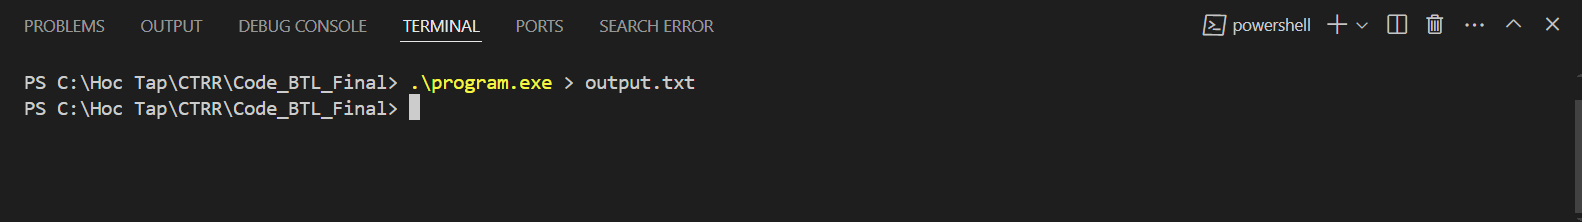
\includegraphics[width=16cm]{terminal.png}
\caption{terminal}
\label{fig:terminal}
\end{figure}

\begin{figure}[h!]
\centering
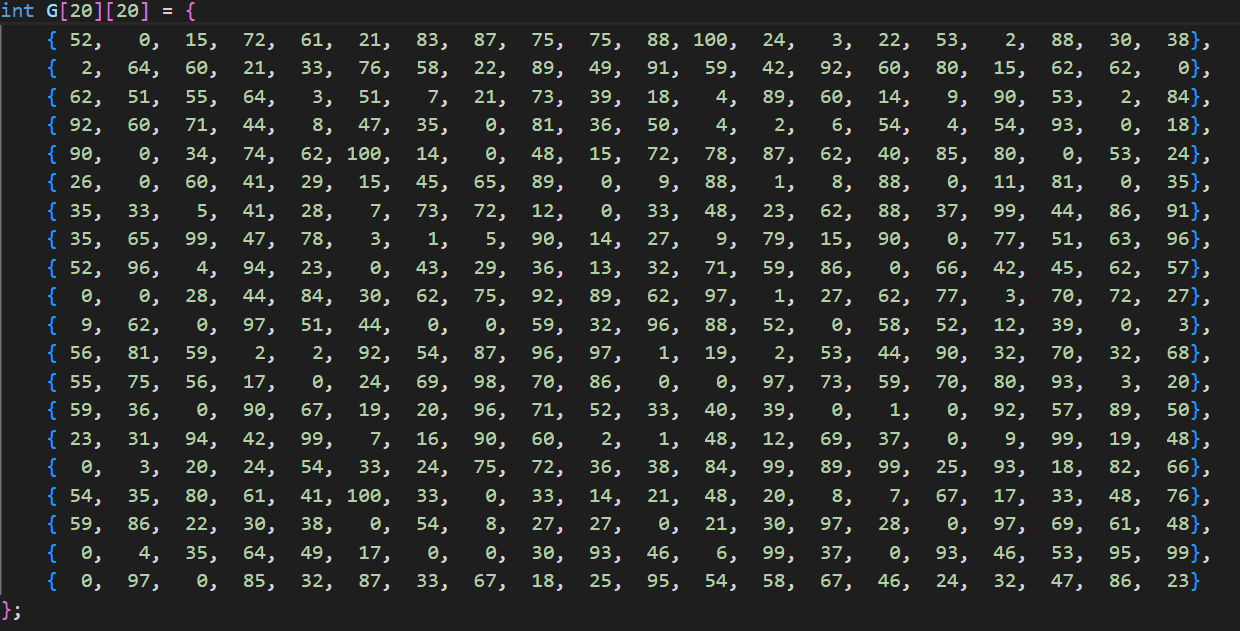
\includegraphics[width=16cm]{input.png}
\caption{Matrix input in file main.cpp}
\label{fig:input}
\end{figure}

\begin{figure}[h!]
\centering
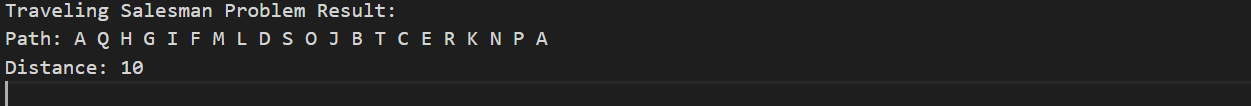
\includegraphics[width=16cm]{output.png}
\caption{Output}
\label{fig:output}
\end{figure}
\vspace{1cm}
\newpage

\section{Conclusion}

This report presents the Branch and Bound method for solving the Traveling Salesman Problem (TSP). This method is a combinatorial optimization technique, notable for its ability to find optimal solutions without the inefficient trial of all possibilities.

\subsection{Highlights}
The Branch and Bound method has proven extremely effective in reducing the search space through its pruning mechanism, which helps eliminate routes that cannot provide an optimal solution. This is particularly important when dealing with problems involving a large number of cities, where the number of permutations can increase exponentially.

\subsection{Applications and Limitations}
Branch and Bound is not only useful for the TSP but can also be applied to many other combinatorial optimization problems. However, it is important to note that the effectiveness of this method can significantly decrease when the input size increases to a certain threshold—this requires more advanced techniques or integration with heuristics to maintain applicability.

\subsection{Future Directions}
Combining Branch and Bound with other advanced algorithms such as genetic algorithms or simulated annealing could extend its capability to solve larger and more complex problems. Continued research in this field not only improves the efficiency of the algorithm but also contributes to the overall theory of optimization.

\textbf{Conclusion:}
Through the study and application of the Branch and Bound method, we find that it is a powerful tool, especially when used in suitable problems. Continued development and adjustment of this method will be key to addressing future optimization challenges.

\newpage
\section*{References}
\begin{enumerate}
    \item Nhánh và Cận - Branch and Bound, Viblo. Available at: \url{https://viblo.asia/p/nhanh-va-can-branch-and-bound-Qbq5QBPEKD8}.
    \item Introduction to Branch and Bound, Geeks for Geeks. Available at: \url{https://www.geeksforgeeks.org/introduction-to-branch-and-bound-data-structures-and-algorithms-tutorial/}.
\end{enumerate}



\end{document}
